\section{The tuberculosis pathway}
\label{sec:tb}

\begin{figure*}[t]
\centering
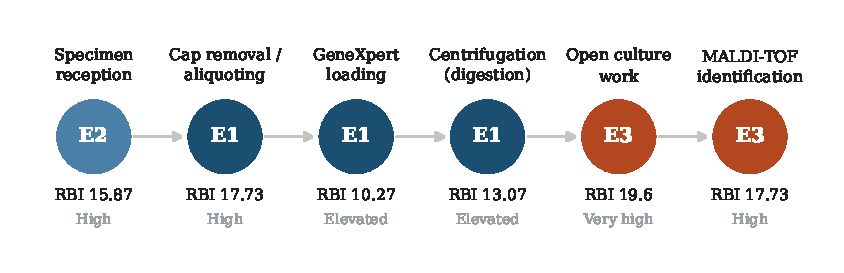
\includegraphics[width=0.98\textwidth]{figures/fig3_tb_pathway.pdf}
\caption{The bench steps a pulmonary tuberculosis specimen passes through, in
the order it meets them. Every step is scored against the low-dose inhalational
profile, which is the profile such a specimen presents, so the indices differ
from the primary-profile column of Table~\ref{tab:inventory}. Marker colour
and label give the evidence grade.}
\label{fig:tb}
\end{figure*}

A sputum specimen from a patient with suspected pulmonary tuberculosis is the
clearest case in this inventory, for three reasons: the organism is
transmissible at low inhaled dose, the specimen may carry a high burden, and
the pathway is long. Figure~\ref{fig:tb} follows one specimen through six of
the seven steps.

\subsection{Every step on the pathway is Elevated or higher}

Scored against the low-dose inhalational profile, the six steps range from
10.27 to 19.60 on the 1--25 index. None falls in the Low or Moderate bands.
This is a different picture from the primary-profile column, where four of the
same steps sit at Moderate or below, and the difference is entirely
attributable to the assumption about the organism rather than to anything about
the procedures.

The practical reading is that a tuberculosis specimen converts the ordinary
pre-analytical bench into elevated-risk work without changing a single physical
action. Specimen reception scores 15.87 and cap removal 17.73 on this pathway,
figures comparable to MALDI-TOF identification, and both of those steps are
routinely performed in general processing areas rather than in the containment
suite that the culture work attracts.

\subsection{The strongest result in the inventory}

Banada and colleagues measured viable bioaerosol at each stage of the
cartridge-based assay workflow \cite{banada2010}. Neither sample preparation
nor automated cartridge processing produced any culturable bioaerosol. In the
same study, preparation of smears for acid-fast microscopy produced 16 and
325~CFU\,m$^{-3}$.

Three things make this result unusually valuable. It is direct measurement of
the clinical procedure, not a surrogate. It is measurement of a procedure
against the procedure it displaces, in one study, under comparable conditions.
And its subject is a respiratory specimen carrying the organism of interest,
rather than a spiked model.

For a tuberculosis programme the implication is favourable and should be stated
plainly: on the only measurement available, replacing smear microscopy with
cartridge-based molecular testing reduces measured bioaerosol release from
detectable to undetectable at that step. Few biosafety interventions have
evidence of that quality behind them.

\subsection{What the result does not establish}

The reassurance is specific and should not be generalised.

The measurement was obtained with the sample reagent used as specified. The
manufacturer specifies a reagent-to-sputum ratio, a dispensing method and a
contact time, and this brief treats all three as part of the control, because
the source read for this release does not establish which of them carries the
inactivation or how far performance degrades when the reagent is used
incorrectly. An earlier draft of this work attributed the safety case to
contact time alone and to a bench timer; that attribution was not supportable
from the source and has been withdrawn. Until the primary methods are read in
full, the honest statement is that correct reagent use as a whole is the
control, and the laboratory should verify all three elements rather than
timing alone.

The result also covers only the molecular testing step. It says nothing about
the reception, aliquoting, digestion and centrifugation, culture and
identification steps that the same specimen passes through, and
Figure~\ref{fig:tb} shows that those steps carry either no measurement or
incident evidence only. A laboratory that has adopted cartridge-based testing
has improved one step of six on measured evidence. The others are unchanged.

\subsection{Implications for tuberculosis laboratory practice}

Three statements are supported by the inventory.

First, the molecular testing step is not where the remaining tuberculosis
bench risk sits, and effort directed there has a low ceiling. Where a cabinet
is available, open transfer should occur within it; where one is not, the
measured evidence supports benchtop loading provided the sample reagent is used
as specified. This brief states that without qualification, because withholding
it would push laboratories without a cabinet toward performing the step with no
guidance at all.

Second, the pre-analytical steps are under-controlled relative to their scores
on this pathway. Reception and aliquoting of respiratory specimens flagged for
mycobacterial investigation score in the High band and are commonly performed
on an open bench in a general processing area.

Third, culture work remains the dominant risk and the recommendation for it is
unchanged and well supported: a certified Class~II cabinet for all
manipulation, with certification on a defined schedule.

\subsection{Why this supports a laboratory survey}

A survey of tuberculosis laboratory practice is a scarce instrument: there are
a limited number of questions a laboratory will answer carefully. Those
questions should be spent where the answer is both actionable and currently
unknown.

The inventory identifies where that is. It is not the molecular testing step,
where practice is good and the evidence is strong. It is the pre-analytical
handling of respiratory specimens before anyone has established what they
contain, the cover-open maintenance conditions on automated equipment that no
study has characterised, and the certification status of the cabinets on which
the culture-step recommendation entirely depends.
Section~\ref{sec:survey} sets out items accordingly.
